\begin{figure}
    \centering
    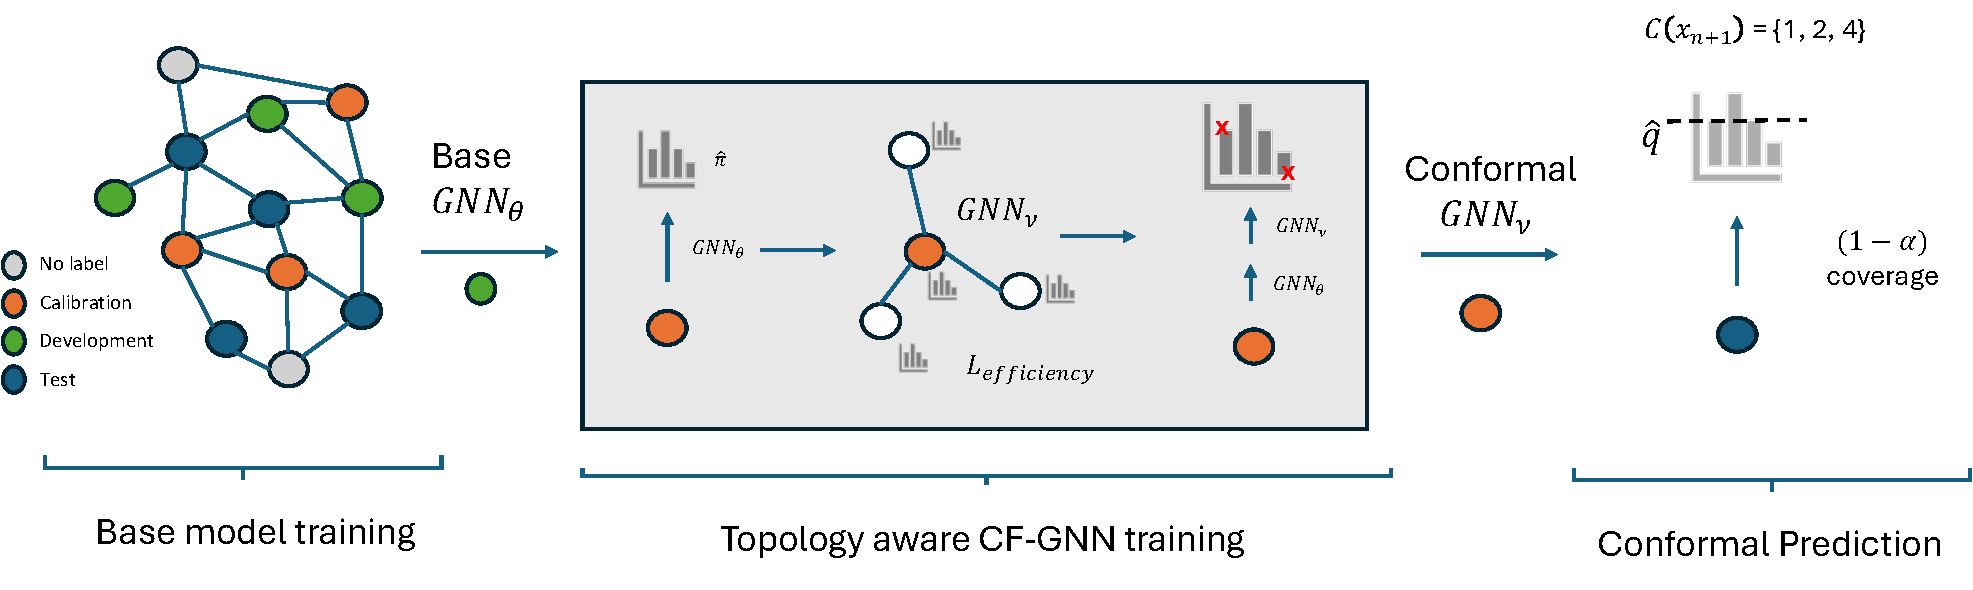
\includegraphics[width=\linewidth,alt={CF-GNN three stage training procedure.}]{graphConformal/figures/CFGNN.pdf}
    \caption{Procedure for training CF-GNN. First (left), the base model is trained on the training set. Then, (middle) the CF-GNN is trained to maximize efficiency over the calibration set. Finally , (right) the non-conformity scores from the combined models are used to generate the prediction sets.}
    \label{fig:conformalized_gnn}
\end{figure}

Conformalized GNN (CFGNN)~\citep{huang2024uncertainty} is a GNN-based approach for conformal prediction.
The authors observed that inefficiencies are correlated between nodes having similar neighborhood topology in a graph setting.
They use a GNN during the calibration phase, which is trained to correct the scores output from the base model such that the corrected scores maximize the efficiency of the conformal prediction.
For classification-based losses, CFGNN utilizes the fact that all steps in the conformal prediction stage for computing the prediction sets (non-conformity score computation, quantile computation, thresholding) can be expressed as differentiable operations.
Thus, a GNN can be trained directly using efficiency as a loss function.
Figure~\ref{fig:conformalized_gnn} provides a high-level overview of the CFGNN approach.

\noindent \textbf{CFGNN Implementation Improvements}
The choice of the conformal loss during calibration and test plays an important role in determining the overall performance of the CFGNN.
\citet{huang2024uncertainty} use a TPS loss for the calibration phase and the non-randomized APS loss for constructing the final prediction sets.
Our preliminary experiments (Figure~\ref{fig:CFGNN:preliminary}) with replacing the APS loss with a randomized version demonstrated that these losses must be tuned carefully to ensure that the CFGNN is able to improve upon the base models non-conformity scores.
Some improvements shown in CFGNN (Figure~\ref{fig:CFGNN:preliminary}, right) get nullified when the randomized APS loss is used (left).

Additionally, CFGNN uses full batch training which makes it unable to scale for larger graphs.
We implemented a batched version of CFGNN to ensure that it can be used for larger graphs.
Finally, to speed up computation, we allow the use of cached outputs from the base model rather than having to sample neighbors for both the base model and the CFGNN.
Algorithm~\ref{alg:cfgnn:catching} shows these improvements in the CFGNN implementation.
We cache the output of the base $\text{GNN}_\theta$ prior to running the CFGNN training loop, allowing the sampling of $m$ layers of message passing graphs rather than $m + l$ layers required by the baseline CFGNN.
In addition, we control the batch size $b$ when sampling neighbors.
These changes significantly speeds up the computation for CFGNNs (see Section~\ref{sec:conformal:results:cfgnn:runtime} for speedup results).
\begin{algorithm}
    \caption{CFGNN batching + caching implementation}\label{alg:cfgnn:catching}
    \begin{algorithmic}[1]
    \State $\text{GNN}_{\theta}$ \Comment{$l$ layer base GNN, with pretrained, fixed weights}
    \State $\text{GNN}_{\phi} \gets \Call{\text{RandomInitialization}}{\phi}$ \Comment{$m$ layer trainable CFGNN}
    \If{cache\_base}
        \State $\gX \gets \text{GNN}_{\theta}(\gG, \gX)$ \Comment{Compute base model output}
    \EndIf
    \Procedure{CFGNNTrainStep}{$\calib, \gG, \gX$}
        \State $\gB \gets \Call{\text{SampleBatch}}{\calib, b}$ \Comment{batch size $b$ is $|\calib|$ for base CFGNN}
        \If{cache\_base}
            \State{$\text{CFFeats, CFMsgGraphs} \gets \Call{\text{ NeighborSampler}}{\gB, m, \gX}$}
        \Else
            \State{$\text{Feats, MsgGraphs} \gets \Call{\text{NeighborSampler}}{\gB, l + m, \gX}$}
            \State{$\text{CFFeats} \gets \text{GNN}_\theta(\text{Feats}, \text{MsgGraphs}_{0, \dots, m-1})$}
            \State{$\text{CFMsgGraphs} \gets \text{MsgGraphs}_{m, \dots, m+l-1}$}
        \EndIf
        \State $\text{scores} \gets \text{GNN}_{\phi}(\text{CFFeats}, \text{CFMsgGraphs})$
        \State $\gL \gets \Call{\text{ConformalLoss}}{\text{scores}, \gB}$
        \State $\Call{\text{UpdateWeights}}{\text{GNN}_\phi, \gL}$
    \EndProcedure
    \end{algorithmic}
\end{algorithm}


\begin{figure}
    \centering
    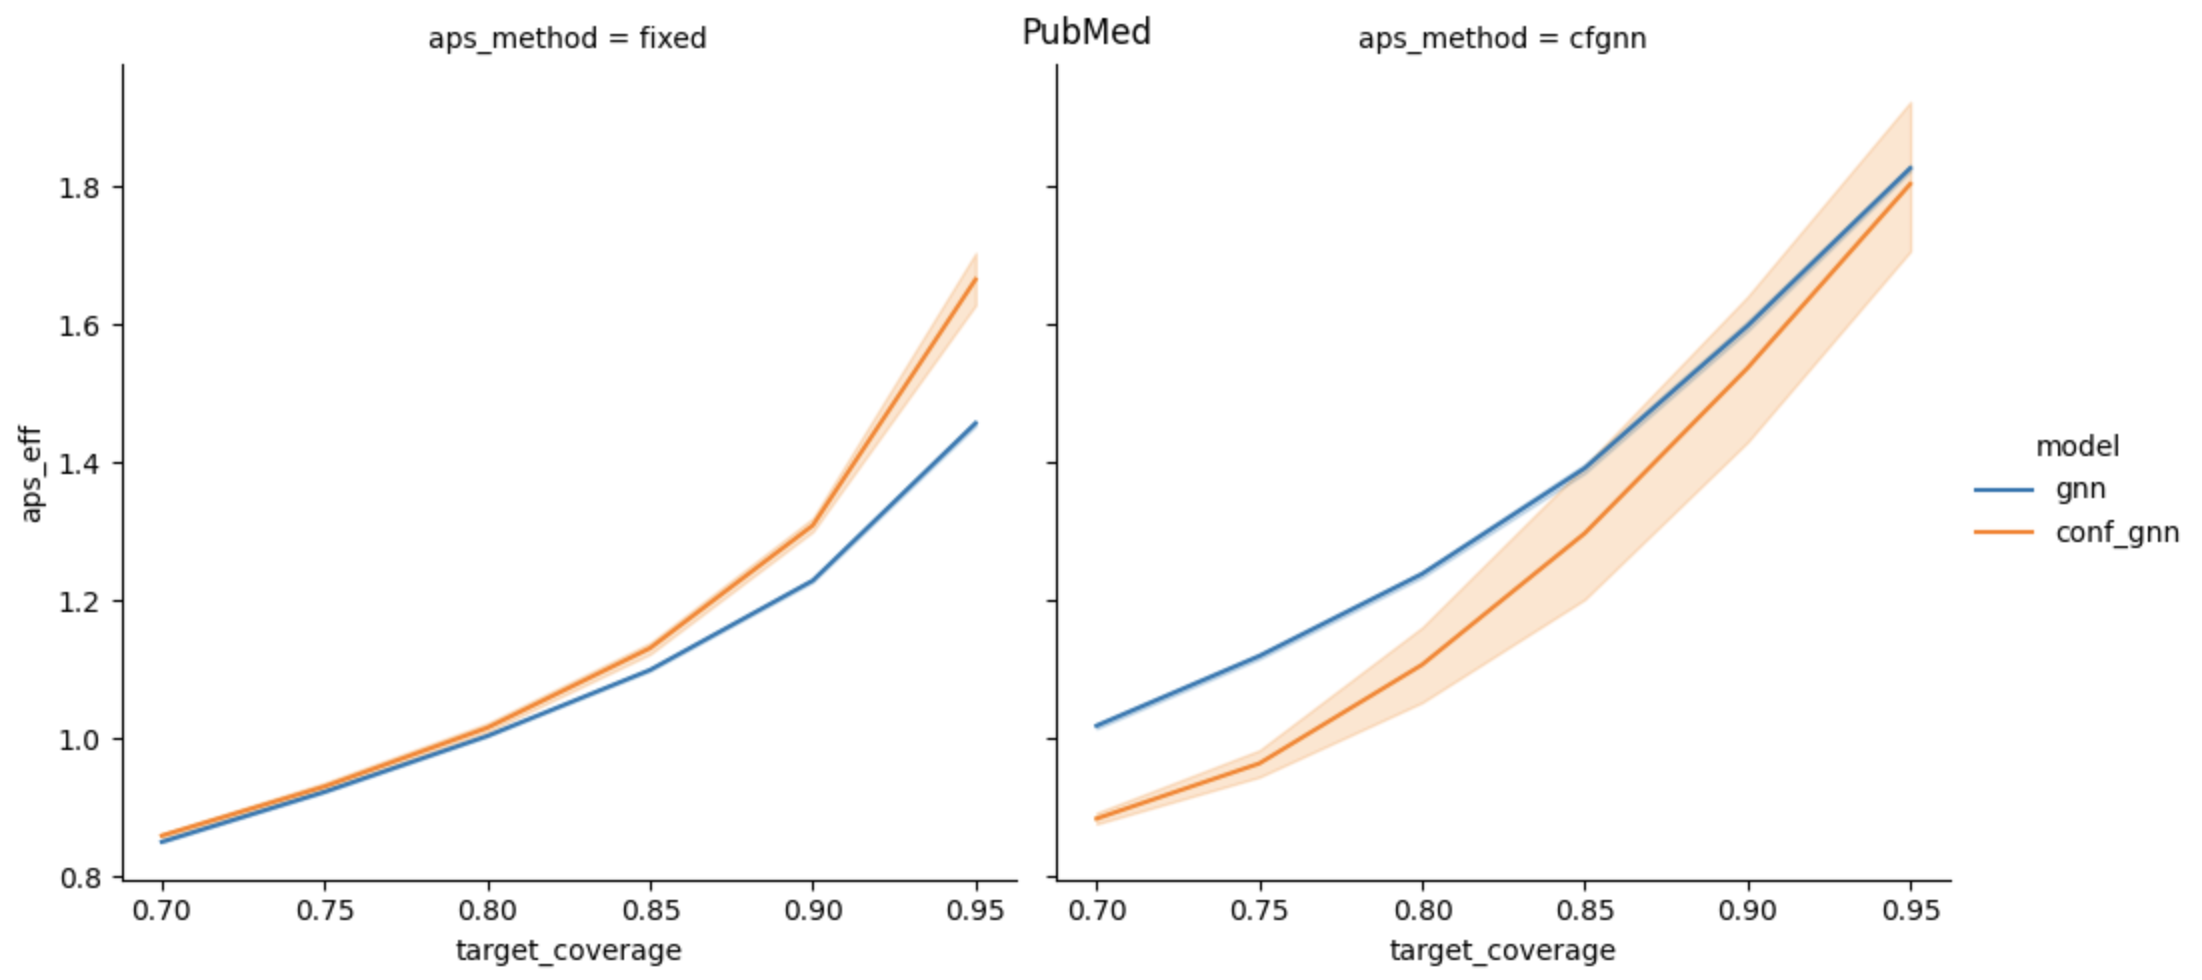
\includegraphics[width=0.8\linewidth,alt={Preliminary results on effciency comparison with APS vs CFGNN.}]{graphConformal/figures/PubMed_CF.png}
    %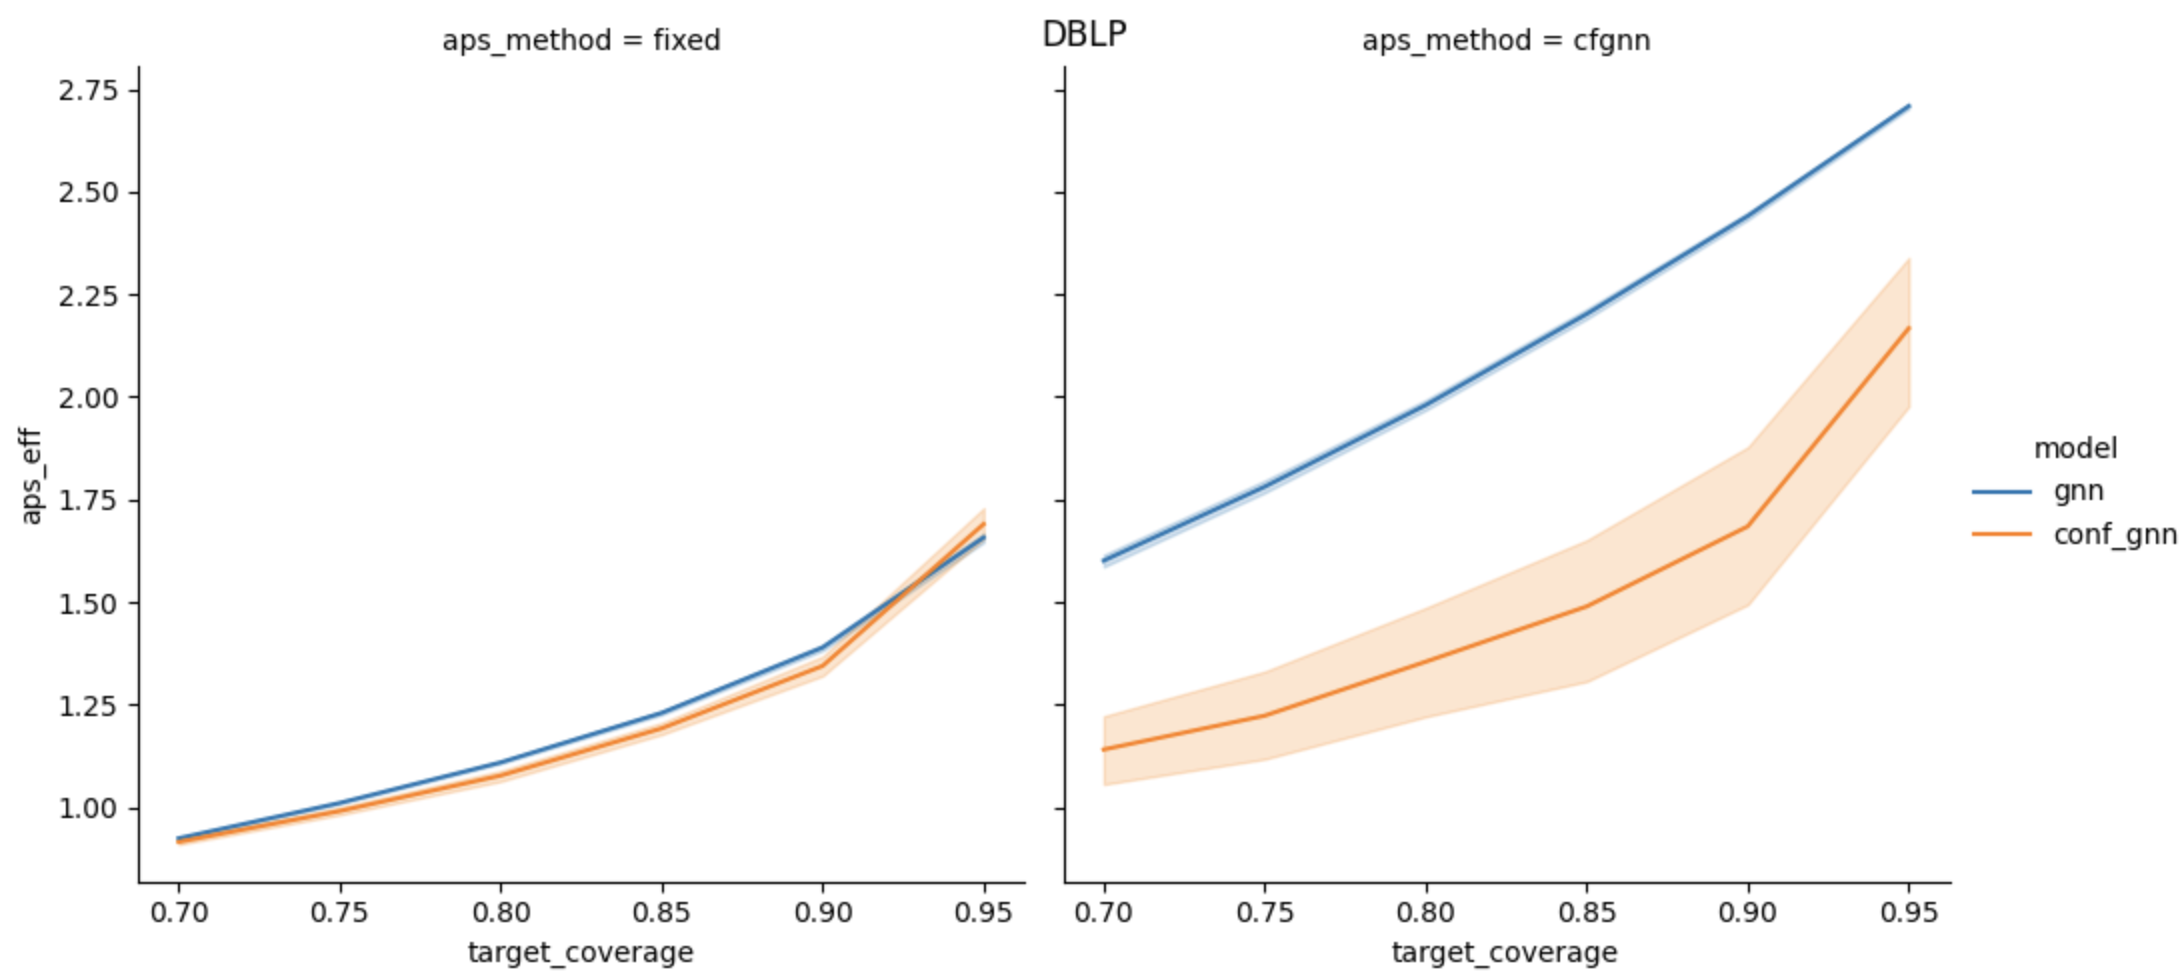
\includegraphics[width=0.7\linewidth]{graphConformal/figures/DBLP_CF.png}
    \caption{Comparing the efficiency (average output set size) for the base model and the CFGNN on the Pubmed dataset. The plot on the left uses the fixed version of the APS score (with randomized sets) while on the right uses the non-randomized version.}
    \label{fig:CFGNN:preliminary}
\end{figure}
